% Compile from this directory:
%   xelatex main.tex
\documentclass[aspectratio=169,10pt]{ctexbeamer}

\usepackage{booktabs}
\usepackage{amsmath,amssymb}
\usepackage{array}
\usepackage{makecell}
\usepackage{tikz}
\usetikzlibrary{arrows.meta,positioning,calc}
\usepackage{adjustbox}

\definecolor{fsspec}{HTML}{FDEBD0}
\definecolor{fscommit}{HTML}{E5F6EA}
\definecolor{fsmiss}{HTML}{F8E8E8}
\newcommand{\Work}{W}
\newcommand{\Xfer}{X}
\newcommand{\paperfig}[2][0.68]{%
  \begin{adjustbox}{max width=0.98\textwidth,max height=#1\textheight,center}
    \input{../tex_new/#2}%
  \end{adjustbox}}

\definecolor{fsblue}{HTML}{1F4E79}
\definecolor{fsorange}{HTML}{C45911}
\definecolor{fsgreen}{HTML}{1B7A3A}
\definecolor{fspurple}{HTML}{5B2C6F}
\definecolor{fsgray}{HTML}{5D6D7E}
\definecolor{fslight}{HTML}{E8F1F8}
\definecolor{fsred}{HTML}{B00020}
\definecolor{fsgain}{HTML}{0B6E4F}
\definecolor{tblhead}{HTML}{E7EEE6}

\newcommand{\sys}{\textsf{ForkServe}}
\newcommand{\fsplus}{\textsf{ForkServe+}}
\newcommand{\app}{\textsf{APP}}
\newcommand{\kv}{KV}
\newcommand{\good}[1]{\textcolor{fsgain}{\textbf{#1}}}
\newcommand{\bad}[1]{\textcolor{fsred}{#1}}
\newcommand{\src}[1]{\vspace{0.3em}{\scriptsize\color{fsgray}#1\par}}

\usefonttheme{professionalfonts}
\setbeamertemplate{navigation symbols}{}
\setbeamertemplate{itemize item}{\small\textcolor{fsblue}{\ensuremath{\bullet}}}
\setbeamertemplate{itemize subitem}{\scriptsize\textcolor{fsorange}{\ensuremath{\circ}}}

\setbeamercolor{structure}{fg=fsblue}
\setbeamercolor{normal text}{fg=black,bg=white}
\setbeamercolor{frametitle}{fg=white,bg=fsblue}
\setbeamercolor{title}{fg=fsblue}
\setbeamercolor{subtitle}{fg=fsgray}
\setbeamercolor{block title}{fg=white,bg=fsblue}
\setbeamercolor{block body}{fg=black,bg=fslight}
\setbeamercolor{block title alerted}{fg=white,bg=fsorange}
\setbeamercolor{block body alerted}{fg=black,bg=fslight}
\setbeamercolor{block title example}{fg=white,bg=fsgreen}
\setbeamercolor{block body example}{fg=black,bg=fslight}
\setbeamercolor{author in head/foot}{fg=white,bg=fsblue}
\setbeamercolor{title in head/foot}{fg=white,bg=fsblue}
\setbeamercolor{date in head/foot}{fg=white,bg=fsblue}

\setbeamerfont{frametitle}{size=\large,series=\bfseries}
\setbeamertemplate{frametitle}{%
  \nointerlineskip
  \begin{beamercolorbox}[wd=\paperwidth,sep=0.45em,leftskip=0.6em]{frametitle}%
    \usebeamerfont{frametitle}\insertframetitle
  \end{beamercolorbox}%
}

\setbeamertemplate{footline}{%
  \leavevmode
  \hbox{%
    \begin{beamercolorbox}[wd=.34\paperwidth,ht=2.6ex,dp=1.1ex,leftskip=1em]{author in head/foot}%
      \usebeamerfont{footline}\sys
    \end{beamercolorbox}%
    \begin{beamercolorbox}[wd=.42\paperwidth,ht=2.6ex,dp=1.1ex,center]{title in head/foot}%
      \insertsection
    \end{beamercolorbox}%
    \begin{beamercolorbox}[wd=.24\paperwidth,ht=2.6ex,dp=1.1ex,rightskip=1em plus 1fil]{date in head/foot}%
      \hfill\insertframenumber\,/\,\inserttotalframenumber
    \end{beamercolorbox}%
  }%
}

\setbeamertemplate{title page}{%
  \vspace{1.6em}
  {\usebeamerfont{title}\usebeamercolor[fg]{title}\inserttitle\par}
  \vspace{0.7em}
  {\usebeamerfont{subtitle}\usebeamercolor[fg]{subtitle}\insertsubtitle\par}
  \vspace{1.4em}
  {\small\color{fsgray}\insertauthor\par}
}

\title{\sys}
\subtitle{每页一个问题，一句原因，一组数据对比}
\author{一次 fan-out：trunk 长度 $L$，\,$k$ 条 residual $\ell_i$，最后一条 committed spine}
\date{}

\newcommand{\why}[1]{{\small\textbf{\color{fsgreen}原因.}\ #1}\par\vspace{0.45em}}

\begin{document}

\begin{frame}
  \titlepage
  \vspace{1.1em}
  \begin{columns}[T]
    \begin{column}{0.32\textwidth}
      \textbf{\color{fsblue}问题 1}\\[0.25em]
      {\small Decode-time pruning 为什么省不了 prefill？}
    \end{column}
    \begin{column}{0.32\textwidth}
      \textbf{\color{fsblue}问题 2}\\[0.25em]
      {\small 为什么默认阈值是 $0.15$，不是 $0.45$？}
    \end{column}
    \begin{column}{0.32\textwidth}
      \textbf{\color{fsblue}问题 3}\\[0.25em]
      {\small Expand 快了约 $10\times$，端到端为什么只降一点？}
    \end{column}
  \end{columns}
\end{frame}



\section{背景}

\begin{frame}{一次 fan-out 的钱花在哪三步？}
  \why{只提交一条 spine，但 APC 把 trunk 克隆 $k$ 份，DistServe / Splitwise 把算出的页全部搬走，ESC / Speculative Rejection / DPTS 要等 token 已经在显存里才打分。}
  \begin{columns}[T]
    \begin{column}{0.32\textwidth}
      \begin{block}{Work，GPU prefill}
        \footnotesize 第一次 expand，block 还没进 radix index。
        \[W = kL + \textstyle\sum_i \ell_i\]
      \end{block}
    \end{column}
    \begin{column}{0.32\textwidth}
      \begin{block}{Xfer，connector}
        \footnotesize 被丢掉的 residual 如果已经 \texttt{insert}，也走这条链路。$X$ 与 $W$ 同一批页。
      \end{block}
    \end{column}
    \begin{column}{0.32\textwidth}
      \begin{block}{Decode-to-cut}
        \footnotesize 窗口、$\tau$ 或 mini-step 都在 prefill 之后。这段 decode 剪不掉。
      \end{block}
    \end{column}
  \end{columns}
  \vspace{0.35em}
  {\fontsize{6.2}{7.0}\selectfont
  Yao, Yu, Zhao, Shafran, Griffiths, Cao, Narasimhan. \textit{Tree of Thoughts: Deliberate Problem Solving with Large Language Models.} NeurIPS 2023.\\
  Kwon, Li, Zhuang, Sheng, Zheng, Yu, Gonzalez, Zhang, Stoica. \textit{Efficient Memory Management for Large Language Model Serving with PagedAttention.} SOSP 2023.\\
  Zhong, Liu, Chen, Hu, Zhu, Liu, Jin, Zhang. \textit{DistServe: Disaggregating Prefill and Decoding for Goodput-optimized Large Language Model Serving.} OSDI 2024.\\
  Patel, Choukse, Zhang, Shah, Goiri, Maleki, Bianchini. \textit{Splitwise: Efficient Generative LLM Inference Using Phase Splitting.} ISCA 2024.
  }
\end{frame}

\begin{frame}{ESC 要等到什么时候才停？}
  \why{熵为 0 读的是已经生成完的答案。图中窗口 $w{=}5$、计划样本 $L{=}20$。窗口关不上时，每个样本都已经 prefill，并 decode 到预算。}
  \begin{center}
    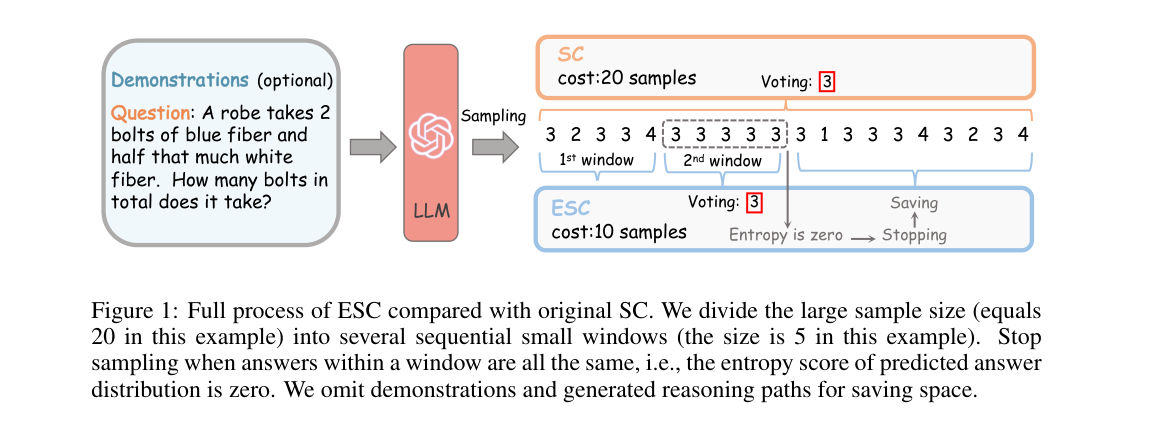
\includegraphics[width=0.90\textwidth]{figs/esc_fig1.png}
  \end{center}
  \src{Li, Yuan, Feng, Pan, Wang, Sun, Wang, Li. \textit{Escape Sky-High Cost: Early-Stopping Self-Consistency for Multi-Step Reasoning.} ICLR 2024. 图：原文 Figure 1.}
\end{frame}

\begin{frame}{Speculative Rejection 在砍分位之前已经付了什么？}
  \why{论文在 partial-reward horizon $\tau{=}256$ 才用 reward model 停掉较低分位 $\alpha$。停掉之前，每条候选的 prefill 和前 $\tau$ 个 token 已经付过。小 $k$ 上 memory-limit 触发器不响。}
  \begin{center}
    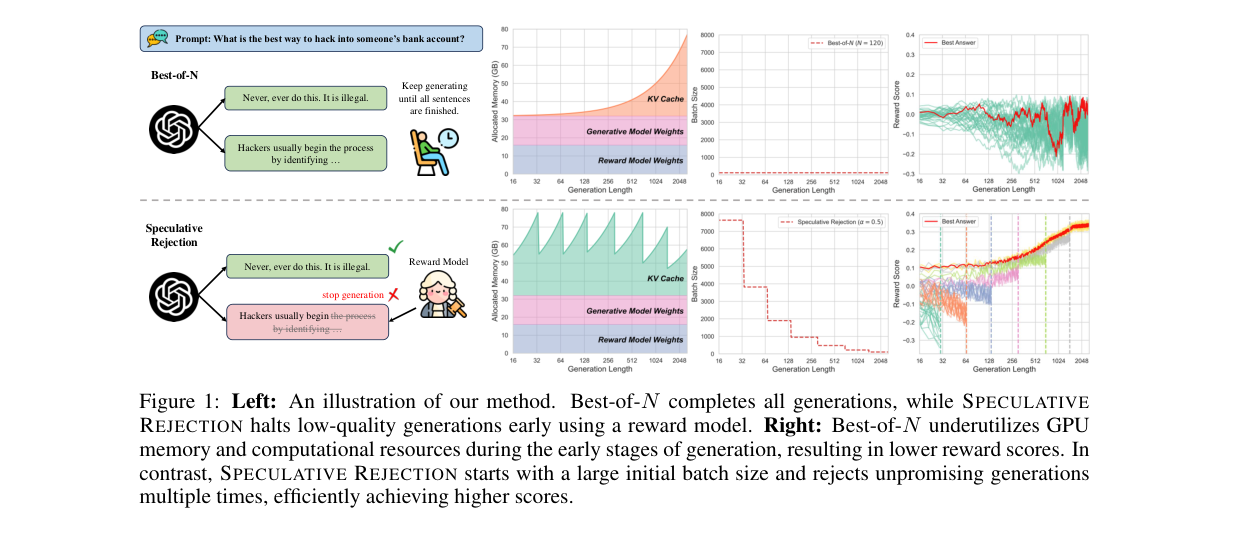
\includegraphics[width=0.92\textwidth,height=0.52\textheight,keepaspectratio]{figs/sr_fig1.png}
  \end{center}
  \src{Sun, Haider, Zhang, Yang, Qiu, Yin, Wang, Bartlett, Zanette. \textit{Fast Best-of-N Decoding via Speculative Rejection.} NeurIPS 2024. 图：原文 Figure 1.}
\end{frame}

\begin{frame}{DPTS 的 early-stop 读的是哪一段 token？}
  \why{每个孩子先生成固定 mini-step，置信度低于 $\theta_{\mathrm{es}}$ 才停。剪枝读的是已经生成的 mini-step。我们复现时这一步是 100 token。}
  \begin{center}
    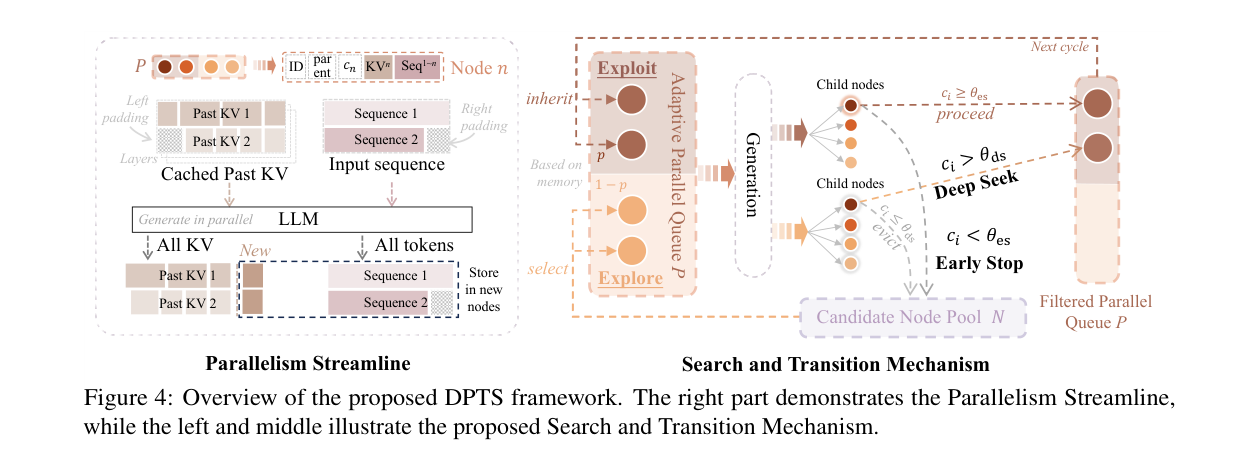
\includegraphics[width=0.86\textwidth]{figs/dpts_fig4.png}
  \end{center}
  \src{Ding, Jiang, Liu, Jing, Guo, Wang, Zhang, Wang, Liu, Du, Liu, Tao. \textit{Dynamic Parallel Tree Search for Efficient LLM Reasoning.} ACL 2025. 图：原文 Figure 4.}
\end{frame}

\begin{frame}{为什么这三篇的 prefill token 一样？}
  \why{分数都来自已经 resident 的 token。剪得越早，decode 越少，prefill 不变。}
  {\footnotesize
  \setlength{\tabcolsep}{6pt}
  \begin{tabular}{@{}lrrrr@{}}
    \toprule
    \textbf{$k{=}16$，host 单独跑} & \textbf{prefill} & \textbf{decode} & \textbf{e2e} & \textbf{any} \\
    \midrule
    ESC & 5008 & 131072 & 17.05\,s & $16/16$ \\
    Speculative Rejection & 5008 & 98304 & 13.14\,s & $16/16$ \\
    DPTS & 5008 & 78336 & 11.86\,s & $16/16$ \\
    \bottomrule
  \end{tabular}}
  \src{Qwen3-8B，GSM8K，$n{=}16$，$D{=}512$，$\mathrm{tp}{=}1$，四张 A100-40GB。\texttt{logs/prune\_ablation\_thresh/all.json}，2026-10-01，policy $=$ base。}
\end{frame}

\section{设计}

\begin{frame}{Admission 和 decode-time pruning 差在哪一步？}
  \why{Decode-time 的分数在 prefill 和 \texttt{insert} 之后。这里先读 draft：loop 不进 kernel，connector 只搬 $\mathrm{Keep}$。}
  \begin{center}
  \begin{tikzpicture}[
      font=\scriptsize\sffamily,
      >=Latex,
      box/.style={draw=fsblue!60, rounded corners=1.5pt, fill=white, align=center,
                  inner sep=2.5pt, minimum height=0.72cm, font=\scriptsize\sffamily},
      badbox/.style={box, draw=fsred!70, fill=fsmiss},
      goodbox/.style={box, draw=fsgreen!70!black, fill=fscommit},
      arr/.style={-{Latex[length=1.6mm]}, line width=0.5pt, draw=fsblue!70},
      lab/.style={font=\tiny\sffamily, text=fsgray}
    ]
    \node[font=\scriptsize\bfseries, anchor=west, text=fsred] at (0,2.55) {Decode-time pruning $+$ P/D};
    \node[badbox] (a1) at (1.15,1.55) {$k$ residuals};
    \node[badbox] (a2) at (3.55,1.55) {prefill\\[-1pt]\tiny all};
    \node[badbox] (a3) at (5.85,1.55) {decode prefix\\[-1pt]\tiny window / $\tau$ / step};
    \node[box] (a4) at (8.25,1.55) {score};
    \node[box] (a5) at (10.15,1.55) {drop};
    \node[badbox] (a6) at (12.35,1.55) {\texttt{insert} all};
    \draw[arr] (a1)--(a2)--(a3)--(a4)--(a5)--(a6);
    \node[lab, anchor=west] at (0.15,0.85) {$W{=}X{=}kL{+}\sum_i\ell_i$。被丢掉的孩子已经进过 kernel，也已经过了 connector。};

    \node[font=\scriptsize\bfseries, anchor=west, text=fsgain] at (0,-0.05) {这里：admission，然后只搬 $\mathrm{Keep}$};
    \node[goodbox] (b1) at (1.15,-1.05) {$k$ residuals};
    \node[goodbox] (b2) at (3.45,-1.05) {draft score\\[-1pt]\tiny $\tau_{\mathrm{pre}}$};
    \node[box, fill=black!4] (b3) at (5.85,-1.85) {loop $\in\Lambda$\\[-1pt]\tiny $W{=}X{=}0$};
    \node[box, fill=fsspec] (b4) at (5.85,-0.25) {其他低分\\[-1pt]\tiny probe $t_0$};
    \node[goodbox] (b5) at (8.35,-1.05) {prefill miss\\[-1pt]\tiny 只留 $\mathrm{Keep}$};
    \node[goodbox] (b6) at (10.85,-1.05) {\texttt{insert} $\mathrm{Keep}$};
    \node[goodbox] (b7) at (13.15,-1.05) {decode\\[-1pt]\tiny spine};
    \draw[arr] (b1)--(b2);
    \draw[arr] (b2.south) -- (b3.north);
    \draw[arr] (b2.north) -- (b4.south);
    \draw[arr] (b4.east) -- ++(0.35,0) |- (b5.north);
    \draw[arr] (b2.east) -- (b5.west);
    \draw[arr] (b5)--(b6)--(b7);
    \node[lab, anchor=west] at (0.15,-2.45)
      {Index 0 永远在 $\mathrm{Keep}$。$s'_i\ge\tau$ 才从 $t_0$ 续到预算 $D$。$X=\sum_{i\in\mathrm{Keep}}W_i$。};
  \end{tikzpicture}
  \end{center}
\end{frame}

\begin{frame}{一条规则怎么同时决定 $W$ 和 $X$？}
  \why{先看 radix 命中 $m_i$。整段命中不进 kernel；部分命中只算 miss；重复 loop 丢掉；其余低分只探前缀；过线才整段 prefill。Index 0 只能是 HS、HP 或 PF。}
  \paperfig[0.55]{fig_dragon.tex}
  \src{论文图。绿页在 $H$，橙页是 prefill，灰页是 withheld。}
\end{frame}

\section{结果}

\begin{frame}{Prefill pruning 比这三个 host 省在哪里？}
  \why{Loop 的分数约 $0.02$，低于 $0.15$，进 kernel 之前丢掉。策略分数约 $1.0$，留下。Admission 不读 host 的切点，所以三个 host 的 prefill 一起下降。ESC 省得最多，因为它本来要把 loop decode 到窗口结束。}
  {\footnotesize
  \setlength{\tabcolsep}{5pt}
  \begin{tabular}{@{}lrrrr@{}}
    \toprule
    \textbf{$k{=}16$} & \textbf{prefill} & \textbf{e2e，单独} & \textbf{e2e，$+\tau_{\mathrm{pre}}{=}0.15$} & \textbf{any} \\
    \midrule
    ESC & $5008\to 3848$ & 17.05\,s & \good{14.13\,s} & $16/16$ \\
    Speculative Rejection & $5008\to 3848$ & 13.14\,s & \good{12.47\,s} & $16/16$ \\
    DPTS & $5008\to 3848$ & 11.86\,s & \good{11.49\,s} & $16/16$ \\
    \bottomrule
  \end{tabular}}
  \src{同一 JSON。$k{=}8$ 上 SR 和 DPTS 单独跑是 $15/16$，加上 $0.15$ 后是 $16/16$。ESC 的 decode token 从 131072 降到 98304。}
\end{frame}

\begin{frame}{为什么默认是 $0.15$，不是更快的 $0.45$？}
  \why{$0.45$ 把分数约 $0.22$ 的 illegal text 和 loop 一起丢掉。$k{=}16$ 上还 admit 8 条，精度守住；$k{=}4$ 和 $k{=}8$ 上不够。}
  {\footnotesize
  \setlength{\tabcolsep}{6pt}
  \begin{tabular}{@{}lrrrr@{}}
    \toprule
    & \textbf{prefill} & \textbf{admit} & \textbf{ESC e2e} & \textbf{any} \\
    \midrule
    $k{=}16$，base & 5008 & 16 & 17.05\,s & $16/16$ \\
    $k{=}16$，$\tau_{\mathrm{pre}}{=}0.15$ & 3848 & 12 & 14.13\,s & $16/16$ \\
    \good{$k{=}16$，$\tau_{\mathrm{pre}}{=}0.45$} & \good{2768} & \good{8} & \good{10.92\,s} & \good{$16/16$} \\
    \midrule
    $k{=}8$，$\tau_{\mathrm{pre}}{=}0.45$ & 1448 & 4 & \multicolumn{2}{r}{\bad{any $14/16$}} \\
    $k{=}4$，$\tau_{\mathrm{pre}}{=}0.45$ & 732 & 2 & \multicolumn{2}{r}{\bad{any $14/16$}} \\
    \bottomrule
  \end{tabular}}
  \src{$k{=}16$、$\tau_{\mathrm{pre}}{=}0.45$ 上 SR 是 $10.80$\,s，DPTS 是 $10.90$\,s，都是 $16/16$。$k{=}4$ 的 $0.15$ 是 $15/16$。\texttt{prune\_ablation\_thresh}。}
\end{frame}

\begin{frame}{为什么不能把低分全部挡在 prefill 前？}
  \why{Loop 可以在 kernel 前丢。Illegal text 要先 decode $t_0$ 再打分，否则对的分支也被丢掉。}
  {\footnotesize
  \setlength{\tabcolsep}{6pt}
  \begin{tabular}{@{}lrr@{}}
    \toprule
    \textbf{MATH-500，$n{=}32$，$\tau{=}0.45$} & \textbf{any} & \textbf{时间} \\
    \midrule
    $k{=}16$，full fan-out & $20/32$ & 104.1\,s \\
    $k{=}16$，一刀切丢掉全部 $s{<}\tau$ & \bad{$13/32$} & \bad{52.1\,s} \\
    \good{$k{=}16$，probe $t_0{=}128$} & \good{$20/32$} & \good{72.2\,s} \\
    $k{=}16$，连 loop 也 probe & $20/32$ & 74.4\,s \\
    $k{=}8$，full fan-out & $15/32$ & 52.5\,s \\
    \good{$k{=}8$，probe $t_0{=}64$} & \good{$16/32$} & \good{42.0\,s} \\
    \bottomrule
  \end{tabular}}
  \src{$k{=}16$、$t_0{=}128$ 的 decode token 从 524288 降到 393216。Grow 行来自 2026-10-01 的 shard JSON；full 与一刀切来自论文 tab:grow。}
\end{frame}

\begin{frame}{P/D 分离之后，pruning 少搬了多少？}
  \why{Connector 搬的是已经 prefill 的页。$\mathrm{Keep}$ 定在 \texttt{insert} 之前，丢掉的 residual 不进这条链路。}
  {\footnotesize
  \setlength{\tabcolsep}{8pt}
  \begin{tabular}{@{}lrrrr@{}}
    \toprule
    & \textbf{APC} & \textbf{P/D} & \textbf{\sys} & \textbf{\fsplus} \\
    \midrule
    Prefill tokens $W$ & \bad{11520} & \bad{11520} & 3840 & \good{2592} \\
    Connector tokens $X$ & 0 & \bad{11520} & 0 & \good{32} \\
    Fan-out & 139\,ms & \bad{162\,ms} & 47\,ms & \good{31.4\,ms} \\
    \bottomrule
  \end{tabular}}
  \src{控制面代价模型，不是 GPU wall clock。10 sessions，$k{=}4$，$L{=}256$，$\ell{=}32$。论文 tab:app。DistServe、Splitwise、PagedAttention 的完整引用在背景页。}
\end{frame}

\begin{frame}{三轮 ToT 的 expand 为什么比 APC 快？}
  \why{三轮合计 192 条 residual，\fsplus{} 只 prefill 48 条。Connector 只搬赢家的 miss。}
  {\footnotesize
  \setlength{\tabcolsep}{8pt}
  \begin{tabular}{@{}lrrrr@{}}
    \toprule
    \textbf{Expand ms / 题} & \textbf{4B GSM8K} & \textbf{4B Game24} & \textbf{8B GSM8K} & \textbf{8B Game24} \\
    \midrule
    APC & 429 & 435 & 597 & 598 \\
    \sys & 83 & 87 & 94 & 94 \\
    \fsplus & \good{55} & \good{53} & \good{58} & \good{56} \\
    \bottomrule
  \end{tabular}}
  \src{\texttt{logs/tot\_mt}，2026-09-29，$n{=}16$，$k{=}4$，$\mathrm{tp}{=}2$，\texttt{fanout\_ms}/16。\fsplus{} / APC 是 $7.9$--$10.6\times$。}
\end{frame}

\begin{frame}{Expand 快了约 $10\times$，端到端为什么只降一点？}
  \why{端到端里还有两步 32-token decode。发出的 token 几乎不变时，端到端几乎不变。}
  {\footnotesize
  \setlength{\tabcolsep}{7pt}
  \begin{tabular}{@{}lrrrr@{}}
    \toprule
    & \textbf{APC 端到端} & \textbf{\fsplus{} 端到端} & \textbf{APC token} & \textbf{\fsplus{} token} \\
    \midrule
    8B GSM8K & 2.48\,s & \good{1.91\,s} & 3594 & \good{2485} \\
    8B Game24 & 2.15\,s & \good{1.52\,s} & 2943 & \good{1750} \\
    4B GSM8K & 1.66\,s & 1.63\,s & 3421 & 3334 \\
    \bottomrule
  \end{tabular}}
  \src{同一批 \texttt{tot\_mt}。4B GSM8K 的 token 几乎没变，端到端就几乎没变。Qwen3-8B GSM8K 的 \texttt{transfer\_tokens} 是 1402。}
\end{frame}

\begin{frame}{剪完之后，做对的题还在吗？}
  \why{丢掉的是低分 loop。GSM8K 上 4B 持平，8B 少 1 题。Game24 上少做无效分支，做对的次数上升。}
  {\footnotesize
  \setlength{\tabcolsep}{8pt}
  \begin{tabular}{@{}lrrr@{}}
    \toprule
    \textbf{三轮 ToT，$n{=}16$} & \textbf{APC} & \textbf{\sys} & \textbf{\fsplus} \\
    \midrule
    Qwen3-4B GSM8K & $15/16$ & $15/16$ & $15/16$ \\
    Qwen3-8B GSM8K & $16/16$ & $15/16$ & $15/16$ \\
    Qwen3-4B Game24 & $6/16$ & \good{$8/16$} & \good{$9/16$} \\
    Qwen3-8B Game24 & $9/16$ & $9/16$ & \good{$10/16$} \\
    \bottomrule
  \end{tabular}}
  \src{同一批 \texttt{tot\_mt}，one problem per generate。}
\end{frame}

\begin{frame}{只 admit 一条为什么伤精度？}
  \why{没有 score 模式时，app 不按分数留一半，把对的分支也丢掉了。}
  {\footnotesize
  \setlength{\tabcolsep}{8pt}
  \begin{tabular}{@{}lrrrr@{}}
    \toprule
    \textbf{$k{=}16$，$\tau{=}0.45$} & \textbf{admit} & \textbf{prefill} & \textbf{ESC} & \textbf{SR} \\
    \midrule
    app，无 score & \bad{1} & \bad{414} & \bad{$11/16$} & \bad{$9/16$} \\
    app，score & \good{8} & \good{2768} & \good{$16/16$} & \good{$16/16$} \\
    \bottomrule
  \end{tabular}}
  \src{\texttt{logs/prune\_ablation\_wide/all.json}。GSM8K，Qwen3-8B，$n{=}16$。}
\end{frame}

\begin{frame}{少占的 \kv{} 换成了多少吞吐？}
  \why{Spine 比 APC 短，同一块显存里能多放树，decode 饱和之后吞吐上去，TTFT 更晚越过 $1$\,s。}
  {\footnotesize
  \setlength{\tabcolsep}{8pt}
  \begin{tabular}{@{}lrr@{}}
    \toprule
    \textbf{DeepSeek-R1，GSM8K} & \textbf{APC} & \textbf{\sys} \\
    \midrule
    测到的 peak & 761 token & \good{561 token} \\
    $8$\,GiB 里的并发树 & 76 & \good{103} \\
    饱和 decode & 48640 token/s & \good{65920 token/s} \\
    $1$\,s P99 TTFT & 448 QPS 越过 & \good{512 QPS 仍是 $0.81$\,s} \\
    \bottomrule
  \end{tabular}}
  \src{论文测到的 peak 与并发扫描。}
\end{frame}

\begin{frame}{三个问题，各用一组数回答}
  \begin{enumerate}
    \item \textbf{为什么三篇的 prefill 一样？} 分数来自已经 resident 的 token。$k{=}16$ 时 ESC、Speculative Rejection、DPTS 的 prefill 都是 5008。加上 $\tau_{\mathrm{pre}}{=}0.15$ 后是 3848，ESC 从 17.05\,s 到 14.13\,s，仍是 $16/16$。
    \vspace{0.55em}
    \item \textbf{为什么默认是 $0.15$？} $k{=}16$ 上 $0.45$ 更快（ESC 10.92\,s，仍是 $16/16$），但 $k{=}4$ 和 $k{=}8$ 掉到 $14/16$。MATH-500 上一刀切是 $13/32$，$t_0{=}128$ 回到 $20/32$，104.1\,s 到 72.2\,s。
    \vspace{0.55em}
    \item \textbf{Expand 快了，端到端为什么只降一点？} 8B GSM8K 的 expand 从 597\,ms 到 58\,ms，端到端从 2.48\,s 到 1.91\,s，因为发出 token 从 3594 降到 2485。4B GSM8K 的 token 从 3421 到 3334，端到端从 1.66\,s 到 1.63\,s。
  \end{enumerate}
\end{frame}

\end{document}
